\chapter{Технологический раздел}

В качестве языка программирования был выбран язык Haskell.  

\section{Синтаксический анализатор}
Парсер выполняет преобразование текста, записанного на языке Пролог, во внутреннее представление, удобное для дальнейшей работы. Синтаксический анализатор разработан с использование библиотеки \texttt{parsec}.

Для разработки синтаксического анализатора требовалось описать грамматику языка при помощи типов.

\lstinputlisting[caption = {Описание программы}, label={lst1:syntax},language=Haskell, firstline=6, lastline=37]{../src/Language/Prolog/Syntax.hs}

Чтобы разобрать текст программы, необходимо описать, как разобрать любую его структуру. Например, при помощи пакета \texttt{parsec}, чтобы проверить, является ли строка числом, необходимо написать следующий код, представленный в листинге \ref{lst2:syntax}.

\lstinputlisting[caption = {Парсер целого числа}, label={lst2:syntax},language=Haskell, firstline=214, lastline=225]{../src/Language/Prolog/Parser.hs}

В листинге \ref{lst3:syntax} представлен код, необходимый, чтобы получить число, как описанный в листинге \ref{lst2:syntax} тип.

\lstinputlisting[caption = {Парсер структуры языка}, label={lst3:syntax},language=Haskell, firstline=16, lastline=32]{../src/Language/Prolog/Parser.hs}

Подобные действия необходимо выполнить для каждого типа.

\section{Алгоритм унификации}
Алгоритм унификации на языке Haskell представлен в листинге \ref{lst4:unifi}.
\lstinputlisting[caption = {Алгоритм унификации}, label={lst4:unifi},language=Haskell, firstline=282, lastline=301]{../src/Language/Prolog/Algorithm.hs}

Функция принимает в качестве аргументов два терма. Возвращаемым значением, в случае успешной унификации, будет новая цель или подстановка.

\section{Резольвента}
Резольвента описывается при помощи типа данных, приведенной в листинге \ref{lst4:resolv}.
\lstinputlisting[caption = {Резольвента}, label={lst4:resolv},language=Haskell, firstline=39, lastline=41]{../src/Language/Prolog/Algorithm.hs}

Она представляет собой список, каждый элемент которого хранит два значения: заголовок и тело правила. Заголовка может не быть, в случае если это вопрос.

\section{Доказательство}
В листинге \ref{lst4:proof} показан шаг обработки текущей цели.
\lstinputlisting[caption = {Доказательство}, label={lst4:proof},language=Haskell, firstline=112, lastline=145]{../src/Language/Prolog/Algorithm.hs}

В первую очередь проверяется резольвента. Если она пуста, то возвращается выработанная подстановка. Если все цели из текущего правила закончились, то переход к целям из тела следующего правила.
Если встречено отсечение, то продолжается поиск решений в данной ветке, но вместе с найденными результатами возвращается метка отсечения.
Далее вызывается обработчик для текущего терма. Стандартный обработчик, представлен в листинге \ref{lst4:default}.
\lstinputlisting[caption = {Доказательство}, label={lst4:default},language=Haskell, firstline=200, lastline=223]{../src/Language/Prolog/Algorithm.hs}

В данном обработчике выполняется попытка унификации текущей цели со всеми возможными правилами. В случае успешной унификации происходит преобразование резольвенты для каждой отдельной ветки. Если в какой-то момент встречается метка отсечения, и она соответствует текущему терму, то следующие ветки в списке отбрасываются.


\section{Пример работы программы}
Для программы нахождения факториала, приведенной в листинге \ref{lst:pr1}, построено дерево, изображенное на рисунке .
\lstinputlisting[caption = {Факториал}, label={lst:pr1},language=Prolog]{../p1.pro}
\begin{figure}[H]
	\centering{ 
		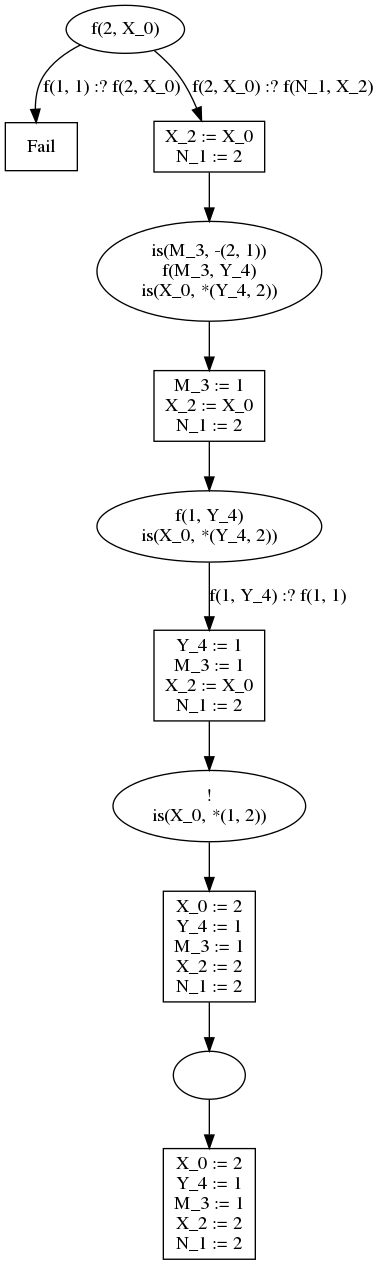
\includegraphics[width=0.4\textwidth]{../fact.png}
		\caption{Дерево поиска решения для факториала}
		\label{uc:1}}
\end{figure}
 
Дерево для быстрой сортировки даже 3 элементов получается слишком большим, чтобы была возможность его вставить сюда. Тем не менее, для программы, приведенной в листинге \ref{lst:pr3}, результат сортировки верный.
\lstinputlisting[caption = {Быстрая сортировка}, label={lst:pr3},language=Prolog]{../p5.pro}

